\documentclass{article}
\usepackage[utf8]{inputenc}
\usepackage{amsmath}
\usepackage{amsfonts}
\usepackage{hyperref}
\DeclareMathOperator*{\argmax}{arg\,max}
\DeclareMathOperator*{\argmin}{arg\,min}

\usepackage{graphicx}

\usepackage{array}
\newcolumntype{C}[1]{>{\centering\arraybackslash\hspace{0pt}}m{#1}}

\usepackage{float}

\setlength{\parindent}{0cm}

\title{Udacity Multiagent Project}
\author{Thomas Lecat}
\date{April 2021}

\begin{document}

    \maketitle


    \section{Environment}\label{sec:environment}

    The environment is described as Markov Decision Process $(S, A, R, p, \gamma)$ with unknown dynamics.
    The goal is to approximate the optimal policy $\pi^*$ that maximizes the upcoming cumulative reward in every state.

    The environment represents two agents playing tennis.
    The action space $A$ of each agent is continuous and consists in 2 actions in the $[-1, 1]$ range.


    \section{Agent}\label{sec:agent}

    \subsection{Multi-agent DDPG}\label{subsec:ddpg}


    A modified version of the \href{https://arxiv.org/abs/1509.02971}{DDPG} agent is implemented as the base solution.

    We follow the paradigm of centralized training and decentralized execution.

    DDPG uses two distinct neural networks: \\

    A "critic" network parameterized by $\theta^Q$ seek to approximate the optimal $Q$ value $Q^*$, defined as:
    \[
        Q^*(s, a, a_{other}) = \max_{\pi} \mathbb{E}_{\pi} (\sum_{t} \gamma^t r_t | S=s, A^{a_0}_0=a, A^{a_1}_0=a_{other}),  \forall (a, a_{other}, s) \in A^2 \times S
    \]
    where $A^{a_0}_t$ and $A^{a_1}_t$ represent the actions of the first and second agents respectively at step $t$.
    The network takes the current observation and action of the agent as well as the action of the other agent as input. It outputs a single value.\\

    A deterministic "actor" network parameterized by $\theta^\mu$ that approximates the function $\argmax_a{Q(\cdot|s)}$.
    It takes the current observation as input.
    The weights of the actor are shared between agents.\\

    The loss function of the critic is defined as the mean squared TD error of the Bellman optimality equation:
    \[
        \mathcal{L}_{critic}(\theta^Q) = \mathbb{E}_{s, a, a_{other}, r, s'} \big[((r + \gamma Q(s', \mu'(s'| \theta^{\mu'}), a_{other}| \theta^{Q'}) - Q(s, a, a_{other}| \theta^Q))^2\big]
    \]
    where $\theta^{Q'}$ and $\theta^{\mu'}$ are the parameters of target networks which are slowly updated towards their respective local networks at every training step.
    The target networks makes the TD target $r + \gamma Q(s', \mu'(s'| \theta^{\mu'}), a_{other}| \theta^{Q'})$ independent from the parameters $\theta^Q$,
    which stabilizes the training.\\

    The loss function of the actor strives to maximise the $Q$ value:
    \[
        \mathcal{L}_{actor}(\theta^{\mu}) = - \mathbb{E}_{s, a_{other}} Q(s, \mu(s | \theta^\mu), a_{other} | \theta^Q)
    \]\\

    The losses are minimized by Adam optimizers, a variant of the Stochastic Gradient Descent algorithm.
    At each step, the gradient is approximated from a minibatch of experiences ${(s, a, a_{other}, r, s', d)_i}$.
    To avoid a strong correlation between the steps of the minibatch, transitions are stored in a large replay buffer
    during rollouts and then sampled uniformly.


    \section{Hyperparemeters}\label{sec:hyperparemeters}

    The actor network is composed of 2 fully connected layers, with respectively 256 and 128 neurons.
    The 3 last local observations of the agent are stacked and form the input of the network.
    The actor optimizer is Adam with a learning rate of $10^{-3}$.

    The critic network is composed of 2 fully connected layers, with respectively 256 and 128 neurons.
    The output of the first layer and the action are concatenated before flowing into the second layer.
    The critic optimizer is Adam with a learning rate of $10^{-3}$.\\

    To increase exploration, random noise created by an Ornstein-Uhlenbeck process is added to the actions during rollouts.\\

    The table below summarizes the main hyperparameters:

    \begin{tabular}{ |p{5cm} C{1cm}|p{3cm}| }
        \hline
        \multicolumn{3}{|c|}{Hyperparameters} \\
        \hline
        actor learning rate                & $\alpha^\mu$ & 1e-03     \\
        \hline
        critic learning rate               & $\alpha^Q$   & 1e-03     \\
        \hline
        discount factor                    & $\gamma$     & 0.99      \\
        \hline
        target networks update coefficient & $\tau$       & 0.006     \\
        \hline
        buffer size                        &              & 1,000,000 \\
        \hline
        batch size                         &              & 128       \\
        \hline
        critic weight decay                &              & 0         \\
        \hline
        Update frequency (number of steps) &              & 1         \\
        \hline
        Number of Adam steps per update    &              & 1         \\
        \hline

    \end{tabular}


    \section{Results}\label{sec:results}

    We plot the mean reward per agent per episode during training:

    \begin{figure}[H]
        \centering
        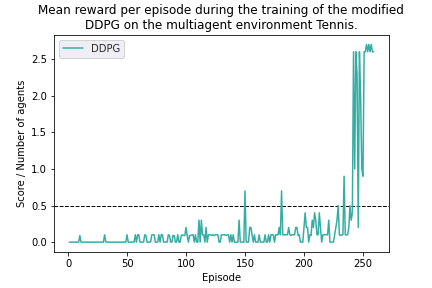
\includegraphics[scale=0.5]{results/mean_reward_per_episode.png}\label{fig:figure}
    \end{figure}

    The environment is solves after 260 episodes.


    \section{Next steps}\label{sec:next-steps}

    As a next step, other multi-agent RL algorithms such as \href{http://proceedings.mlr.press/v80/rashid18a.html}{Q-Mix}
    could be tested on this problem and compared to the current implementation.

    Hyperparemeters could also be further tuned using strategies such as
    \href{https://github.com/hyperopt/hyperopt}{HyperOpt} or
    \href{https://deepmind.com/blog/article/population-based-training-neural-networks}{Population Based Training}.

\end{document}
